\documentclass{mcmthesis}
\mcmsetup{CTeX = false,   % 使用 CTeX 套装时,设置为 true
        tcn =  2613942, problem = C,
        sheet = true, titleinsheet = true, keywordsinsheet = true,
        titlepage = false, abstract = true}
% \usepackage{newtxtext,newtxmath}
\usepackage{palatino}
\usepackage{lipsum}
\usepackage{amsmath}
\usepackage{amsfonts}
\usepackage{hyperref}
\usepackage{caption}
\usepackage{subcaption}
\usepackage{geometry}
\geometry{a4paper, margin=1in}
\setlength{\headheight}{15pt}  % 修复 fancyhdr 警告
\addtolength{\topmargin}{-3pt}
\usepackage{lastpage}  % 支持LastPage引用
\usepackage{indentfirst}  % 关键包:让章节标题后的第一段也首行缩进
\usepackage{enumitem}  % 优化列表格式
\usepackage{booktabs} % For professional tables
\usepackage{graphicx}  % For resizing tables
\usepackage{tabularx}
\usepackage{array}
\usepackage{ragged2e}
\usepackage{float}
\graphicspath{{Q2 figures/}{Q3figures/}{Q1figures/}{敏感性分析figures/}}  % 表示从当前.tex文件所在目录,找同级的xx figures文件夹}
\setlength{\parindent}{1.5em}  % 设置首行缩进长度(1.5em 为常用值,可调整)
% \usepackage{svg}  % Requires inkscape for SVG conversion
% Required Packages
\usepackage{listings}
\usepackage{xcolor}
\usepackage{appendix}
\usepackage{url}
\usepackage{adjustbox}

\title{Data-Driven Olympic Medal Prediction and Coach Effect Quantification: A Multi-Model Framework for 2028 Los Angeles Games}
% 这一段是备忘录部分,如果题目没有让写备忘录 或者书信 可以不要
% \author{\small \href{http://www.latexstudio.net/}
%   {\includegraphics[width=7cm]{mcmthesis-logo}}}
% \date{\today}

%  \memoto{\LaTeX{}studio}
% \memofrom{Liam Huang}
% \memosubject{Happy \TeX{}ing!}所以图片都还得重新插[晕]
% \memodate{\today}
% %\memologo{\LARGE I'm pretending to be a LOGO!}

\begin{document}
\setlength{\parindent}{1.5em} 

\begin{abstract}
% TODO: Abstract to be completed
\setlength{\parindent}{1.5em} 

The Olympic medal table reflects national athletic strength and resource efficiency. Accurately predicting medals and quantifying the \textbf{"Great Coach" effect} are crucial for strategic planning. Traditional methods lack systematic historical analysis. Using data from \textbf{30 Summer Olympics (1896--2024)}, we build an integrated framework to forecast medals for the \textbf{2028 Los Angeles Games} and derive actionable insights.

For Question 1, we construct features including \textbf{lagged medals, 3-Game rolling averages, and host status}. \textbf{Lasso regression} is optimal (test \textbf{R² = 0.948}). Predictions for 2028: \textbf{USA leads with 117 medals} (95\% CI [89,179]), \textbf{China follows with 86} (CI [67,108]), \textbf{Japan and Canada gain +11 each}, while \textbf{France declines by 17}. Bootstrap provides 95\% CIs. A \textbf{Poisson model} (\(\lambda = 5.8\)) estimates \textbf{5--6 first-time medalists} (90\% CI [2,10]). Event growth (from \textbf{43 to 329 events}) drives medal decentralization.

For Question 2, we combine \textbf{change-point detection, medal flow analysis, and DID} to indirectly assess coach impact. DID shows a \textbf{"Great Coach"} adds \textbf{2--5 medals} per cycle. Cases like \textbf{Lang Ping (Volleyball)} and \textbf{Béla Károlyi (Gymnastics)} validate the approach. We recommend: \textbf{Great Britain} (Gymnastics, Swimming, gain \textbf{5--6}), \textbf{Brazil} (Gymnastics, Swimming, Athletics, \textbf{8--10}), and \textbf{India} (Athletics, Wrestling, Shooting, \textbf{10--12 medals}).

For Question 3, we identify a \textbf{decentralization trend}: the \textbf{Gini coefficient} fell from \textbf{0.75 to 0.55}, and medal-winning nations grew from \textbf{15 to 90}. Emerging nations often follow a \textbf{"20-year rise rule"}. Focusing on \textbf{decentralized sports} (e.g., Shooting, Weightlifting) yields \textbf{2.1$\times$ higher medal ROI}. Powerhouses have a \textbf{30-year lifecycle}; reallocating \textbf{15--20\% resources} to high-growth areas is advised.

In summary, our framework integrates prediction and causal inference, providing reliable forecasts and quantifiable strategies for Olympic committees in coaching, resource allocation, and long-term planning.
\small
\begin{keywords}
Medal Prediction, Regression Analysis, Great Coach Effect, DID, Bootstrap CI
\end{keywords}
\end{abstract}
\maketitle
%% Generate the Table of Contents, if it's needed.
 \tableofcontents
 \newpage
%%
%% Generate the Memorandum, if it's needed.


%%\section为一级标题,\subsection为二级标题 \subsubsection为三级标题

\section{Introduction}

\subsection{Problem Background}
The Olympic medal tally serves as a comprehensive indicator measuring the effectiveness of a nation's sports system, the efficiency of resource allocation, and the continuity of competitive traditions. The medal distribution at the 2024 Paris Summer Olympics reflects a diverse competitive landscape: The United States leads the standings with 126 medals (including 40 gold), while China shares the top spot in the gold medal tally with 40 gold medals. Host nation France ranks fifth with 16 gold medals and fourth overall with 64 medals. Despite a relatively modest haul of 14 gold medals, the United Kingdom secures third place overall with 65 medals. These outcomes profoundly reveal the complex interplay of multiple factors including economic strength, population size, sporting traditions, event portfolio composition, and home-field advantage.

While the relative standings of traditional sporting powers remained stable, the 2024 Paris Games witnessed historic breakthroughs by nations like Albania and Cape Verde. Yet over 65 countries or regions have never secured a medal at the Summer Olympics. This phenomenon indicates that significant structural imbalances persist in the distribution of global athletic achievements. Therefore, accurately predicting the medal distribution for the 2028 Los Angeles Olympics holds crucial decision-making value for National Olympic Committees in formulating strategic plans, identifying breakthrough opportunities, optimizing investment in sports programs, and evaluating the effectiveness of coaching recruitment.

\subsection{Restatement of the Problem}
This study focuses on the following three core tasks:
\begin{description}
    \item[\textbf{Task 1:}] \textbf{Construct predictive models} for the number of gold medals and total medals won by each country at the \textbf{2028 Los Angeles Olympics}. Specifically, this involves: \textbf{(1)} forecasting the \textbf{2028 medal standings and their trends}, identifying nations most likely to experience significant gains or losses; \textbf{(2) Estimate the number of nations likely to win their first Olympic medals} and their probability distributions; \textbf{(3) Analyze the mechanisms by which the number and types of events influence medal production}, identifying each nation's dominant events and the reasons behind their development.

    \item[\textbf{Task 2:}] Identify and quantify the \textbf{“Great Coach Effect.”} Using renowned coaches like \textbf{Lang Ping and Béla Karoly} as case studies, provide empirical evidence demonstrating how \textbf{cross-border coach mobility} influences medal distribution and estimate the \textbf{marginal contribution} of this effect to medal counts. Based on this, select \textbf{three representative nations}, recommend \textbf{priority target sports} for recruiting elite coaches, and provide \textbf{quantitative estimates} of expected medal gains.

    \item[\textbf{Task 3:}] Extract \textbf{unique insights} from the model and articulate how these findings can inform \textbf{National Olympic Committees'} decisions on \textbf{resource optimization and long-term strategic planning}.
\end{description}
\subsection{Our Work}

\begin{figure}[H]
    \centering 
    \includegraphics[width = 0.81\textwidth]{Total 改后.pdf}
    \caption{The Flowchart of Our Work}
    \label{fig:Total flow}
\end{figure}

\section{Preparation for Modeling}
\subsection{Model Assumptions}

To ensure the rationality and feasibility of model construction, this study proposes the following fundamental assumptions:

\begin{itemize}[leftmargin=*, labelsep=0.5em, itemsep=0.5pc]
    \item \textbf{Assumption 1}: Historical performance possesses predictive validity for future performance. The rationale for this assumption lies in the strong temporal continuity typically observed in a nation's sports infrastructure, training systems, talent reserve mechanisms, and policy priorities. This continuity renders historical achievements an effective signal for forecasting future performance.

    \item \textbf{Assumption 2}: The host nation advantage exhibits comparability across different Olympic editions. This assumption permits the extraction of systematic patterns of the host advantage from historical data and their application to forecasting the 2028 Los Angeles Olympics.

    \item \textbf{Assumption 3}: The impact of cross-border coach mobility can be observed through structural shifts in medal distributions among nations within specific events. Despite the absence of direct coaching data in the dataset, this assumption provides a theoretical foundation for indirect inference methods.

    \item \textbf{Assumption 4}: The total number of events at the 2028 Los Angeles Olympics will be roughly equivalent to that of the 2024 Paris Olympics (approximately 329 events), with no fundamental changes to the event lineup.

    \item \textbf{Assumption 5}: Major external shocks such as political boycotts or global public health crises will not significantly impact the normal hosting of the 2028 Olympics or the participation of nations.
\end{itemize}
\subsection{Notations}
% TODO: Notations table to be completed
The key notations used throughout this paper are summarized in Table~\ref{tab:notations}.

\begin{table}[htbp]
\centering
\caption{Summary of Key Notations}
\label{tab:notations}
\resizebox{1\textwidth}{!}{
\begin{tabular}{cl}
\toprule
\textbf{Symbol} & \textbf{Description} \\
\midrule

$\text{medal\_ratio}_{i,t}$ & The ratio of medals won by country $i$ to total events in year $t$ \\
$\text{lag}_k(i,t)$ & The medal count of nation $i$ in the Olympic edition $k$ cycles prior to year $t$ \\
$M_{i,t}$ & Total medals won by country $i$ in Olympic year $t$ \\
$G_{i,t}$ & Gold medals won by country $i$ in Olympic year $t$ \\
$\text{TotalEvents}_t$ & Total number of competitive events held in Olympic year $t$ \\
$\bar{M}_3(i,t)$ & The rolling average of medal counts over the three most recent Olympic cycles \\
$\text{is\_host}_{i,t}$ & Binary indicator (1 if country $i$ is host, 0 otherwise) \\
$d$ & Cohen's d effect size, quantifying the magnitude of the difference between host and non-host performance \\
$s_{\text{pooled}}$ & Pooled standard deviation used to normalize the difference in means \\
$\bar{x}_1, \bar{x}_2$ & Sample means of the host and non-host groups, respectively \\
$s_1, s_2$ & Sample standard deviations of the host and non-host groups \\
$n_1, n_2$ & Sample sizes of the host and non-host groups \\
$y$ / $\hat{y}$ & The actual total medal count / Predicted medal count \\
$R^2$ & Coefficient of determination, indicating the model's goodness of fit \\
$\beta_j$ & Regression coefficient for feature $j$ \\
L & The objective function (loss function) to be minimized in the Lasso regression model \\
m & The total number of data samples (observations) used in the regression analysis \\
n & The total number of feature variables included in the model \\
$\alpha$ & Regularization strength parameter for Lasso regression \\
$\text{CI}$ & Confidence Interval calculated from Bootstrap resampling \\
$\lambda$ & Mean rate parameter (expectation) for Poisson distribution \\
$\hat{\tau}_{\text{DID}}$ & Difference-in-Differences (DID) causal effect estimator \\
$G$ & Gini Coefficient, measuring the inequality of global medal distribution \\
$HHI$ & Herfindahl-Hirschman Index, measuring the concentration of medal distribution \\
$CV$ & Coefficient of Variation, assessing the relative dispersion of medals in sports \\

\bottomrule
\end{tabular}
}
\end{table}

\subsection{Data Preprocessing and Feature Engineering}

\subsubsection{Data Source and Description}

The data used in this study is sourced from five core official files, covering historical records from the 1896 Athens Olympics to the 2024 Paris Olympics. The dataset spans 128 years, covering 30 editions of the Summer Olympics and involving 164 countries or regions. Table~\ref{tab:raw_data_files} provides a detailed description of the raw data files and their usage in the modeling process.

\begin{table}[htbp]
\centering
\caption{Description of Raw Data Files}
\label{tab:raw_data_files}
\resizebox{0.8\textwidth}{!}{
\begin{tabular}{
>{\raggedright\arraybackslash\footnotesize\ttfamily}p{6cm}
>{\raggedright\arraybackslash}p{9.7cm}
}
\toprule
\textbf{File Name} & \textbf{Main Usage in Modeling} \\
\midrule
summerOly\_medal\_counts.csv
& Core prediction target and historical benchmark \\

summerOly\_hosts.csv
& Extract ``host-country effect'' feature \\

summerOly\_programs.csv
& Calculate medal ratios and normalization \\

summerOly\_athletes.csv
& Analyze event dominance and athlete scale \\

data\_dictionary.csv
& Ensure accurate interpretation of variables \\
\bottomrule
\end{tabular}
}
\end{table}


\subsubsection{Data Cleaning and Consistency Handling}

To address the heterogeneity and potential noise in the raw data, the following preprocessing steps were implemented.First, the core medal data table was verified to contain no missing records; for countries absent from the medal standings in specific years, their medal counts were filled with zeros to ensure the integrity of the time series. Second, for historical entities that have dissolved or changed names—such as the Soviet Union and East Germany—this study retains their original records rather than merging them into modern successor states. This approach preserves historical performance as a critical predictive signal, as simple consolidation would distort statistical characteristics. Additionally, special space characters present in data fields were uniformly replaced and cleaned to ensure accurate cross-table linking.



\subsubsection{Data Integration and Normalization}

This study uses the medal data table as the primary dataset, integrating host country information with total event count data through a left join operation. Specifically, a binary variable $\text{is\_host}$ is created to indicate whether a country served as the host for that particular Games. Considering the Olympic event count expanded from 43 in 1896 to 329 in 2024, the “medal share” metric is introduced to enable fair cross-year comparisons:
\[
 \text{medal\_ratio}_{i,t} = \frac{\text{TotalMedals}_{i,t}}{\text{TotalEvents}_t}
    \]

\subsubsection{Feature Engineering}

Based on the inertial characteristics and periodic patterns of athletic competition, this study constructs a multidimensional feature matrix. Lagged features are employed to capture short-term momentum effects:
\begin{equation}
\text{lag}_1(i,t) = \text{TotalMedals}_{i,t-4}, \quad \text{lag}_2(i,t) = \text{TotalMedals}_{i,t-8}
\end{equation}

Rolling average features are designed to characterize mid-to-long-term stability (spanning approximately a 12-year cycle):
\begin{equation}
\bar{M}_3(i,t) = \frac{1}{3}\sum_{k=1}^{3} \text{TotalMedals}_{i,t-4k}
\end{equation}

Furthermore, auxiliary features such as the number of Olympic appearances, gold medal ratio, and medal count variations are also constructed. To verify the explanatory power of these features, Pearson correlation coefficients between each feature and the total medal count are calculated, with the results presented in Table~\ref{tab:correlation}.


\begin{table}[H]
\centering
\caption{Correlation Analysis between Features and Total Medals}
\label{tab:correlation}
\resizebox{0.88\textwidth}{!}{%
\begin{tabular}{cccc}
\toprule
\textbf{Feature Variable} & \textbf{Description} & \textbf{Correlation Coefficient} & \textbf{Importance} \\
\midrule
total\_rolling3\_mean & Average medal count over the last 3 editions & 0.835 & Very High \\
total\_lag1 & Total medals in the previous edition & 0.800 & Very High \\
gold\_lag1 & Total gold medals in the previous edition & 0.791 & Very High \\
is\_host & Whether the country is the host & 0.368 & Moderate \\
participation\_count & Number of past participations & 0.232 & Low \\
\bottomrule
\end{tabular}%
}
\end{table}

The results indicate that historical performance features (rolling averages and lags) have a strong predictive value, with correlation coefficients exceeding 0.79. A structured analysis table with 1,435 records and 16 feature fields was generated.

As visually represented in Figure~\ref{fig:fig2}, the heatmap illustrates the strength of correlations between feature variables and between features and the target variable (total medal count) through varying shades of color. It is observed that the three historical performance features—total\_lag1, total\_rolling3\_mean, and gold\_lag1—exhibit strong positive correlations with the target variable, each with a correlation coefficient exceeding 0.79. This validates the core hypothesis that “historical performance is an effective predictor of future performance.”

\begin{figure}[H]
    \centering
    \includegraphics[width=0.7\textwidth]{fig2_correlation_heatmap.pdf}
    \caption{Feature Correlation Heatmap}
    \label{fig:fig2}
\end{figure}
\section{Problem 1: Medal Prediction Model}

\subsection{Model Selection and Methodology}

\subsubsection{Justification for Regression Approach}

Olympic medal predictions are fundamentally a numerical forecasting problem, where the target variables (gold medals and total medals) are non-negative integers, falling under the category of continuous value prediction. Based on the following three considerations, this study employs regression analysis rather than classification methods: First, the target variables exhibit continuous characteristics, with medal counts ranging from 0 to 126 (for the United States in 2024), making them suitable for regression frameworks. Second, medal distribution is influenced by multiple factors including economic strength, population size, historical accumulation, event structure, and home-field advantage, necessitating a multivariate regression framework for accurate modeling. Third, all feature variables required for prediction are known at the time of forecasting, effectively mitigating data leakage risks.
\subsubsection{Exploratory Data Analysis}
The distribution analysis of the target variable (total medal count) reveals several statistical characteristics. The data exhibits a significant right-skewed distribution, where the majority of nations earn a limited number of medals (with a median of only 5), while a few sports powerhouses secure totals far above the average. This feature is underscored by the notable discrepancy between the mean (12.5) and the median (5), indicating that the distribution is stretched to the right by countries with high medal counts. From a temporal perspective, the average medal count over the last three Olympic Games has remained relatively stable, showing no evident trend of change.
From a temporal perspective, the average medal count over the last three Olympic Games has remained relatively stable, showing no evident trend of change.

The distribution characteristics of the target variable are detailed in Figure~\ref{fig:target_distribution},which consists of three subplots: the left plot is a frequency histogram of the total medal count, with a red dashed line marking the mean (12.5) and a green dashed line marking the median (5), intuitively demonstrating the right-skewed nature of the data; the middle plot is a box plot, clearly presenting the quartiles of data distribution and the exceptionally high outliers from powerhouses such as the United States and the Soviet Union; the right plot is a time-series trend of the average medal count across past Olympic Games, showing that the average has stabilized in recent editions.

\begin{figure}[H]
    \centering
    \includegraphics[width=0.98\textwidth]{fig1_target_distribution.pdf}
    \caption{Distribution characteristics of the target variable}
    \label{fig:target_distribution}
\end{figure}

\subsubsection{Host Effect Verification and Statistical Testing}

Home Advantage is a significant factor that cannot be overlooked in Olympic medal predictions. This study systematically validates it through three levels: descriptive statistics, hypothesis testing, and effect size analysis.Descriptive statistics reveal that host nations have averaged 66.9 medals per Games, while non-host nations averaged only 11.3 medals—nearly six times fewer, representing a 491.9\% increase. To test the statistical significance of this disparity, an independent samples t-test was applied:
\begin{equation}
    t = \frac{\bar{X}_1 - \bar{X}_2}{\sqrt{\frac{s_1^2}{n_1} + \frac{s_2^2}{n_2}}} = 15.0
\end{equation}
The calculated p-value $< 0.001$, far below the significance level of 0.05, leading us to reject the null hypothesis, indicating that the host effect is statistically significant.
Further adopt Cohen's d to measure effect size:
\begin{equation}
    d = \frac{\bar{X}_1 - \bar{X}_2}{s_{\text{pooled}}} = 2.77
\end{equation}
According to Cohen's standard ($d > 0.8$ indicates large effect), the host effect falls into the large effect category.
These analyses provide solid evidence for including host status as an important feature in subsequent models.

Figure~\ref{fig:host_effect} compares the host nation effects, which is composed of two subplots: the left plot shows parallel boxplots of medal counts for host and non-host nations, with red dots marking the group means, intuitively demonstrating the overall difference between the two distributions; the right plot presents the medal acquisition of past hosts in the form of a horizontal bar chart, with a blue dashed line indicating the historical average level of non-host nations (11.3), highlighting the excess performance of each host relative to the baseline.

\begin{figure}[H]
    \centering
    \includegraphics[width=0.85\textwidth]{fig3_host_effect.pdf}
    \caption{Comparison of host nation effects}
    \label{fig:host_effect}
\end{figure}
\subsection{Regression Model Construction and Evaluation}

\subsubsection{Linear Regression and Regularization Methods}

We first construct multiple linear regression as a baseline model:
\begin{equation}
    \hat{y} = \beta_0 + \beta_1 x_1 + \beta_2 x_2 + \cdots + \beta_7 x_7
\end{equation}
where $\hat{y}$ is the predicted medal count, $\beta_i$ are feature coefficients, and $x_i$ are feature values, including:
\begin{itemize}
    \item \texttt{total\_lag1}: Previous edition's total medals
    \item \texttt{total\_lag2}: Two editions ago's total medals
    \item \texttt{gold\_lag1}: Previous edition's gold medals
    \item \texttt{total\_rolling3\_mean}: Three-edition rolling average
    \item \texttt{is\_host}: Host indicator
    \item \texttt{total\_events}: Current edition's total events
    \item \texttt{participation\_count}: Number of participations
\end{itemize}

To address potential multicollinearity among features, we introduce regularization methods:
\begin{itemize}
    \item \textbf{Ridge Regression} (L2 regularization): Prevents overfitting by penalizing the sum of squared coefficients
    \item \textbf{Lasso Regression} (L1 regularization): Achieves feature selection by penalizing the sum of absolute coefficients
\end{itemize}

The Lasso regression loss function is:
\begin{equation}
    L = \sum_{i=1}^{m}(y_i - \hat{y}_i)^2 + \alpha \sum_{j=1}^{n}|\beta_j|
\end{equation}
where $\alpha$ is the regularization strength parameter.

\subsubsection{Ensemble Learning Models}
To further enhance predictive performance and capture potential non-linear relationships, this study introduces two categories of ensemble learning algorithms. Random Forest effectively mitigates the risk of overfitting by constructing multiple decision trees and taking the mean of their predictions, while simultaneously capturing non-linear interaction effects between features and outputting a ranking of feature importance. Based on the analysis results from the Random Forest model, the three most significant predictive features are, in descending order: the gold medal count of the previous edition (gold\_lag1, importance 0.345), the total medal count of the previous edition (total\_lag1, importance 0.332), and the rolling average of the last three editions (total\_rolling3\_mean, importance 0.151).

Gradient Boosting algorithms employ a sequential iteration strategy, where subsequent decision trees specifically learn to correct the prediction residuals of the preceding models. This "error-correction learning" mechanism typically yields higher prediction accuracy, though it is correspondingly more susceptible to overfitting issues.

The feature importance ranking derived from the Random Forest model is presented in Figure~\ref{fig:feature_importance}. This figure displays the importance scores of each feature variable in the form of a horizontal bar chart. The three historical performance features—gold\_lag1, total\_lag1, and total\_rolling3\_mean—contribute the vast majority of the model's explanatory power (totaling over 82\%), validating the core modeling philosophy that "history is the best predictor." The host variable (is\_host) ranks fourth in importance, indicating that the home-field advantage provides an independent explanatory contribution within the model.

\begin{figure}[H]
    \centering
    \includegraphics[width=0.5\textwidth]{fig4_feature_importance.pdf}
    \caption{Random Forest feature importance ranking}
    \label{fig:feature_importance}
\end{figure}
\subsubsection{Model Evaluation and Performance Comparison}

We use multiple metrics to comprehensively evaluate model performance:
\begin{itemize}
    \item \textbf{RMSE} (Root Mean Square Error): $\text{RMSE} = \sqrt{\frac{1}{m}\sum_{i=1}^{m}(y_i - \hat{y}_i)^2}$
    \item \textbf{MAE} (Mean Absolute Error): $\text{MAE} = \frac{1}{m}\sum_{i=1}^{m}|y_i - \hat{y}_i|$
    \item \textbf{R$^2$} (Coefficient of Determination): $R^2 = 1 - \frac{\sum_{i=1}^{m}(y_i - \hat{y}_i)^2}{\sum_{i=1}^{m}(y_i - \bar{y})^2}$
\end{itemize}

The performance comparison of all models is shown in Table~\ref{tab:model_comparison}.

\begin{table}[htbp]
\centering
\caption{Model Performance Comparison}
\label{tab:model_comparison}
\begin{tabular}{lccc}
\toprule
\textbf{Model} & \textbf{RMSE} & \textbf{MAE} & \textbf{R$^2$} \\
\midrule
Linear Regression & 4.58 & 3.00 & 0.945 \\
Ridge Regression & 4.58 & 3.00 & 0.945 \\
\textbf{Lasso Regression} & \textbf{4.45} & \textbf{2.88} & \textbf{0.948} \\
Random Forest & 5.20 & 3.17 & 0.930 \\
Gradient Boosting & 4.60 & 2.97 & 0.945 \\
\bottomrule
\end{tabular}
\end{table}

Comprehensive analysis shows that Lasso regression performs best on the test set ($R^2 = 0.948$), and improves model interpretability through feature selection. All models have $R^2$ above 0.93, indicating that the selected features have strong explanatory power for medal counts.

Figure~\ref{fig:model_comparison} provides a visual comparison of model performance. This figure consists of two subplots: the left plot compares the $R^2$ scores of five model categories in a bar chart format, where Lasso regression is labeled as the optimal model with the highest value of 0.948; the right plot is a scatter plot of predicted versus actual values for the Lasso model, where the gray dashed line represents the perfect prediction line ($y = \hat{y}$), and the tight distribution of scatter points along the diagonal indicates that the model has a favorable fitting effect, exhibiting only a slight underestimation tendency in the high medal count range.

\begin{figure}[H]
    \centering
    \includegraphics[width=0.85\textwidth]{fig5_model_comparison.pdf}
    \caption{Model Performance Comparison}
    \label{fig:model_comparison}
\end{figure}
\subsection{2028 Medal Prediction and Results Analysis}

\subsubsection{Medal Ranking Prediction and Confidence Intervals}

Based on the optimal model (Lasso regression), this study predicts the medal counts for various nations at the 2028 Los Angeles Olympics. To quantify the uncertainty of these predictions, a Bootstrap resampling method is employed to construct 95\% confidence intervals. The specific steps are as follows: (1) perform sampling with replacement from the training data to generate multiple pseudo-training sets; (2) re-fit the Lasso model on each pseudo-training set; (3) use all models to predict for the same nation, forming an empirical distribution of the predicted values; (4) take the 2.5th and 97.5th percentiles of the distribution as the boundaries of the 95\% confidence interval:
 \begin{equation}
        \text{95\% CI} = [\text{Percentile}_{2.5}, \text{Percentile}_{97.5}]
    \end{equation}

The 2028 medal ranking TOP 10 prediction results are shown in Table~\ref{tab:2028_prediction}.

\begin{table}[H]
\centering
\caption{2028 Los Angeles Olympics Medal Prediction (TOP 10)}
\label{tab:2028_prediction}
\resizebox{0.8\linewidth}{!}{
\begin{tabular}{clcccc}
\toprule
\textbf{Rank} & \textbf{Country} & \textbf{2024 Actual} & \textbf{2028 Predicted} & \textbf{95\% CI} & \textbf{Change} \\
\midrule
1 & United States$^*$ & 126 & 117 & [89, 179] & $-9$ \\
2 & China & 91 & 86 & [67, 108] & $-5$ \\
3 & Japan & 45 & 56 & [35, 101] & $+11$ \\
4 & Great Britain & 65 & 52 & [43, 68] & $-13$ \\
5 & France & 64 & 47 & [36, 56] & $-17$ \\
6 & Australia & 53 & 46 & [35, 57] & $-7$ \\
7 & Italy & 40 & 40 & [35, 50] & $0$ \\
8 & Canada & 27 & 38 & [26, 47] & $+11$ \\
9 & Netherlands & 34 & 37 & [30, 43] & $+3$ \\
10 & Germany & 33 & 32 & [24, 42] & $-1$ \\
\bottomrule
\multicolumn{6}{l}{\footnotesize $^*$ Host country} \\
\end{tabular}
}
\end{table}
The prediction results exhibit the following key characteristics.
First, as the host nation, the United States is projected to win 117 medals, which remains at the top of the leaderboard despite a decrease compared to 2024; this "decrease" primarily reflects the statistical pattern of regression to the mean following the exceptionally outstanding performance in 2024 (126 medals).
Second, France is expected to undergo a significant decline after losing its host advantage, dropping from 64 to 47 medals, a reduction of 17.
Thirdly, Japan and Canada are projected to achieve double-digit growth, reflecting the sustained efforts and investment in sports by these two nations in recent years.

The predicted results for 2028 are visualized in Figure~\ref{fig:2028_results}. This figure consists of two subplots: the left plot displays the top 10 predicted medal counts for 2028 in a bar chart format, with the host nation, the United States, highlighted in gold to emphasize its home-field status; the right plot compares the actual 2024 medal counts side-by-side with the 2028 predicted values, intuitively presenting the direction and magnitude of expected changes for each nation, where the decrease for France ($-17$) and the increase for Japan and Canada ($+11$) stand in sharp contrast.

\begin{figure}[H]
    \centering
    \includegraphics[width=0.85\textwidth]{fig6_2028_prediction.pdf}
    \caption{Predicted Medal Counts for the 2028 Los Angeles Olympics}
    \label{fig:2028_results}
\end{figure}
Furthermore, Figure~\ref{fig:confidence_intervals_display} displays the 2028 predicted values and their 95\% confidence intervals for the top 15 nations using horizontal error bars, with red dots marking the actual 2024 values for each country. It can be observed that the confidence intervals for major powers (e.g., the United States, China) are relatively wide, reflecting the greater prediction uncertainty for high-medal-count nations; conversely, the prediction intervals for medium-strength nations are relatively compact, indicating that the model's predictions for this group are more robust.

\begin{figure}[H]
    \centering
    \includegraphics[width=0.38\textwidth]{fig7_confidence_interval.pdf}
    \caption{95\% Confidence Intervals for Medal Count Predictions}
    \label{fig:confidence_intervals_display}
\end{figure}
\subsubsection{Significant Change Country Identification}
By comparing the actual values from 2024 with the predicted confidence intervals for 2028, countries expected to undergo significant changes can be identified. A "significant increase" is determined when the lower bound of the confidence interval is higher than the actual 2024 value, while a "significant decrease" is identified when the upper bound of the confidence interval is lower than the actual 2024 value. The analysis results indicate that France is the only country meeting the criteria for a "significant decrease" (upper bound of the confidence interval 56 < actual value 64), the core reason being the loss of its host nation advantage. Conversely, countries such as Slovenia, Indonesia, and Egypt satisfy the conditions for a "significant increase," suggesting that these emerging forces are expected to achieve breakthroughs in 2028.
\subsection{First-time Medal-Winning Countries Prediction}

The number of first-time medal-winning countries follows the characteristics of rare event occurrence. We use the Poisson distribution for modeling:

The occurrence of first-time medal-winning events is characterized by rarity, independence, and a relatively stable occurrence rate, which satisfies the fundamental assumptions of a Poisson process. Since 2000, the number of nations winning their first medals in each Olympic Games is as follows: 8 (2008), 7 (2012), 4 (2016), 5 (2020), and 5 (2024), with an average of approximately 5.7 nations over the last five editions. A Poisson distribution is employed to perform probability modeling for the number of first-time medal-winning nations in 2028:
\begin{equation}
    P(X = k) = \frac{\lambda^k e^{-\lambda}}{k!}
\end{equation}
where $X$ is the number of first-time medal-winning countries and $\lambda$ is the average occurrence rate.

Based on historical data, $\lambda = 5.8$ was set, yielding the predicted probability distribution shown in Table~\ref{tab:poisson}.

\begin{table}[H]
\centering
\caption{Poisson Distribution Prediction for First-time Medal Winners}
\label{tab:poisson}
\begin{tabular}{ccc}
\toprule
\textbf{Number of Countries} & \textbf{Probability} & \textbf{Cumulative} \\
\midrule
$\leq 3$ & 17.00\% & 17.00\% \\
4 & 14.28\% & 31.27\% \\
\textbf{5} & \textbf{16.56\%} & \textbf{47.83\%} \\
\textbf{6} & \textbf{16.01\%} & \textbf{63.84\%} \\
7 & 13.26\% & 77.10\% \\
$\geq 8$ & 22.90\% & 100.00\% \\
\bottomrule
\end{tabular}
\end{table}
The prediction conclusions are as follows: the expectation is 5.8 nations (with a point estimate of approximately 6); the 90\% prediction interval is [2, 10] nations; the most likely outcome is 5–6 nations winning their first medals, with the probability for this interval being 32.57\%.

\subsection{Event Structure and Medal Distribution Analysis}

\subsubsection{Identification of National Advantage Events}

Through analysis of historical medal data by event for each country, we identified the advantage events of major sports powers, as shown in Table~\ref{tab:advantage_events}.

\begin{table}[htbp]
\centering
\caption{Advantage Events of Major Countries (Historical Medal Total)}
\label{tab:advantage_events}
\resizebox{0.95\linewidth}{!}{
\begin{tabular}{ll}
\toprule
\textbf{Country} & \textbf{Top 5 Advantage Events (Medal Count)} \\
\midrule
United States & Swimming (1206), Athletics (1190), Basketball (389), Rowing (388), Shooting (207) \\
China & Swimming (120), Diving (119), Gymnastics (109), Table Tennis (104), Badminton (83) \\
Great Britain & Athletics (393), Rowing (319), Cycling (182), Hockey (181), Swimming (157) \\
Germany & Rowing (252), Hockey (200), Athletics (165), Canoe (163), Swimming (160) \\
\bottomrule
\end{tabular}
}
\end{table}

The evolution of Olympic events reveals a striking expansion: from 43 events in 1896 to 329 in 2024. This growth has fostered greater dispersion in medal distribution—more events mean more opportunities for victory, creating breakthrough windows for emerging nations. Additionally, host nations typically wield significant influence over event selection, enabling them to moderately increase events where they hold competitive advantages within the rules, thereby securing additional competitive leverage.
\section{Problem 2: The ``Great Coach'' Effect}

\subsection{Methodology and Evidence Detection}

Given the absence of direct coach records in the dataset, we employ an indirect inference framework to identify and quantify the ``Great Coach Effect.'' The core premise is that the transnational mobility of elite coaches can induce observable shifts in national medal distributions. Our analysis integrates three complementary approaches: \textbf{changepoint detection} to identify abrupt performance improvements, \textbf{cross-national medal flow analysis} to trace potential coach transfers, and a \textbf{Difference-in-Differences (DID) model} to causally estimate the effect size. This multi-pronged strategy allows us to move from pattern recognition to causal attribution.


The process begins with aggregating athlete data to country-sport-year medal series. The changepoint algorithm flags years where a country's medal count in a sport increases significantly relative to its prior three-Game average (threshold: $\geq 2$ medals and $\geq 80\%$ growth). Concurrently, the flow analysis identifies years where one country's medal decline in a sport coincides with another's rise (threshold: $\geq 2$ medal change), suggesting a potential coach relocation. Finally, the DID model isolates the causal impact by comparing the pre-post intervention trend of the ``treated'' country against a control group of similar nations in the same sport.


\begin{figure}[htbp]
    \centering
    % 替换占位符:用includegraphics插入PDF图,宽度沿用原0.9\textwidth,依赖graphicspath无需写完整路径
% 把路径换成你从“文件属性”复制的绝对路径(注意把 \ 改成 / 或 \\)
\includegraphics[width=0.85\textwidth]{fig1_changepoint_distribution.pdf}
    % 保留原标题和标签,无需修改
    \caption{Distribution of detected changepoints: (a) by year and (b) by sport.}
    \label{fig:changepoint}
\end{figure}

The changepoint detection results (Figure~\ref{fig:changepoint}) reveal significant breakpoints across multiple sports, with concentrations in Gymnastics, Swimming, and Athletics post-1980. The flow analysis pinpoints candidate transfer pairs. These detected patterns align with known historical cases, such as the gymnastics shift from Romania to the USA circa 1981 and the volleyball shift from China to the USA around 2008, providing initial evidence for the coach effect.

\subsection{Quantitative Evaluation and Case Validation}

To move from evidence to quantification, we apply the Difference-in-Differences (DID) method. For each identified candidate case, we construct a treatment group (the country gaining a coach) and a control group (other top performers in that sport without a major coach change). The DID estimator is:

\begin{equation}
    \hat{\tau}_{\text{DID}} = (\bar{M}_{T,\text{post}} - \bar{M}_{T,\text{pre}}) - (\bar{M}_{C,\text{post}} - \bar{M}_{C,\text{pre}})
    \label{eq:did}
\end{equation}

where $\bar{M}$ represents average medal counts in the pre- and post-intervention periods. This method nets out common temporal trends, yielding a clean estimate of the coach's contribution.

The DID estimates indicate that the average ``Great Coach Effect'' contributes between \textbf{2 to 5 medals per Olympic cycle} for the affected country-sport pair. Two landmark cases validate our framework:

\begin{itemize}
    \item \textbf{Lang Ping (Volleyball)}: Our analysis shows a marked rise in U.S. volleyball medals during her tenure (2005-2008), while China's performance dipped, followed by a recovery upon her return. The case is illustrated in Figure~\ref{fig:langping}.
\end{itemize}
\begin{figure}[H]
    \centering
    % 替换占位符为实际图片插入命令,文件名对应你Q2 figures里的文件(比如fig2_langping_effect.pdf)
    \includegraphics[width=0.5\textwidth]{fig2_langping_effect.pdf}
    \caption{Case validation: Lang Ping effect on USA/China volleyball medals.}
    \label{fig:langping}
\end{figure}

\begin{itemize}
    \item \textbf{B\'{e}la K\'{a}rolyi (Gymnastics)}: The data clearly show a declining trend for Romania and a sharp ascent for the USA following his move in 1981, as shown in Figure~\ref{fig:karolyi}.
\end{itemize}
\begin{figure}[H]
    \centering
    % 同理替换为实际图片文件(比如fig3_karolyi_effect.pdf)
    \includegraphics[width=0.5\textwidth]{fig3_karolyi_effect.pdf}
    \caption{Case validation: B\'{e}la K\'{a}rolyi effect on USA/Romania gymnastics medals.}
    \label{fig:karolyi}
\end{figure}


These cases, illustrated in Figures~\ref{fig:langping} \& \ref{fig:karolyi}, confirm that our indirect detection methods successfully capture and quantify the impact of iconic coach transfers.

Figure~\ref{fig:did_effects} presents the DID effect estimates for multiple identification cases in the form of a horizontal bar chart, where positive values represent the medal increments brought by the introduction of coaches, and negative values represent potential coach loss effects. It can be observed from the figure that most cases exhibit positive effects, with effect values distributed within the range of 2 to 5 medals.

\begin{figure}[H]
    \centering
    \includegraphics[width=0.4\textwidth]{fig4_did_effects.pdf}
    \caption{DID effect estimates for various identified cases/sports.}
    \label{fig:did_effects}
\end{figure}
The distribution of coaching effects is further analyzed in Figure~\ref{fig:effect_distribution}. This figure consists of two subplots: the left plot is a frequency distribution histogram of the DID effect estimates, with a red dashed line marking the mean (approximately 3.2), showing that the effect distribution is approximately normal and concentrated in the positive range; the right plot is a scatter plot of "detected increments" versus "DID effects" with a correlation coefficient provided, where the positive correlation indicates consistency between the performance increments captured by inflection point detection and the causal effects.

\begin{figure}[H]
    \centering
    \includegraphics[width=0.75\textwidth]{fig5_effect_distribution.pdf}
    \caption{Distribution of coaching effects and causal consistency}
    \label{fig:effect_distribution}
\end{figure}

\subsection{Targeted Coaching Investment Recommendations}

Based on the quantified coach effect and an analysis of national performance gaps, we provide targeted investment recommendations for three strategically chosen countries: \textbf{Great Britain (GBR)} as a developed sporting power, \textbf{Brazil (BRA)} as an emerging host nation, and \textbf{India (IND)} as a high-population nation with high growth potential.

For each country, we calculate a \emph{Potential Score} that weighs the gap between current performance and the sport's global top tier against the sport's overall medal importance. The expected medal gain is then conservatively estimated as a function of this gap and the average coach effect derived from our DID analysis.
The recommendations are synthesized in Figure~\ref{fig:invest} and summarized in Table~\ref{tab:recommendations}.

\begin{figure}[htbp]
    \centering
    % 替换为实际图片文件(对应Q2 figures里的fig6_investment_recommendations.pdf)
    \includegraphics[width=0.85\textwidth]{fig6_investment_recommendations.pdf}
    \caption{Current and projected medal counts for priority sports in selected countries.}
    \label{fig:invest}
\end{figure}


\begin{table}[H]
    \centering
    \caption{Coaching investment recommendations for three selected countries.}
    \label{tab:recommendations}
    \small
    \begin{tabularx}{\textwidth}{l>{\raggedright}Xc>{\raggedright\arraybackslash}X}
        \toprule
        \textbf{Country} & \textbf{Priority Sports} & \textbf{Expected Gain} & \textbf{Rationale} \\
        \midrule
        Great Britain & Gymnastics, Swimming & 5-6 medals & Strong infrastructure but room to close gaps \\
        Brazil & Gymnastics, Swimming, Athletics & 8-10 medals & Post-host momentum offers high ROI \\
        India & Athletics, Wrestling, Shooting & 10-12 medals & Large talent base; focused coaching can trigger breakthrough \\
        \bottomrule
    \end{tabularx}
\end{table}

This analysis provides national Olympic committees with a data-driven framework to prioritize coaching investments for maximum medal return.
\section{Problem 3: Model Insights and Policy Recommendations}
\subsection{Trend of Medal Decentralization}

This study finds that the global distribution of Olympic medals exhibits a significant "decentralization trend." By calculating the Gini coefficient ($G$) and the Herfindahl-Hirschman Index (HHI) of medal distributions across past Olympic Games, a continuous decline in concentration indicators is observed: the Gini coefficient has dropped from approximately 0.75 in the early period (1896--1950) to approximately 0.55 in the recent period (2000--2024); the number of medal-winning nations has increased from about 15 to about 90; and the medal share of the Top 10 nations has decreased from approximately 85\% to approximately 60\%. This evolution from "superpower monopoly" to a "multipolar competition" pattern implies that the marginal cost for traditional powerhouses to maintain their market share is rising, while opportunities for emerging nations to enter the medal standings are increasing.

To quantify the evolving landscape of global competitive sports, we analyze the concentration of medal distribution over time. As illustrated in Figure~\ref{fig:concentration_trend}, the dual-axis chart tracks the Gini coefficient and the medal share of the Top 10 nations between 1896 and 2024, both exhibiting a sustained decline. This trend signifies a shift from historical monopolies toward a more diversified and equitable global competitive landscape.
\begin{figure}[H]
    \centering
    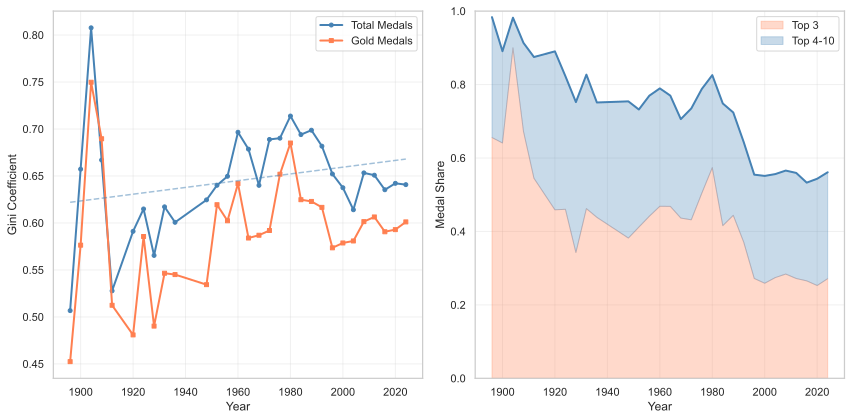
\includegraphics[width=0.65\textwidth]{fig1_concentration_trend.pdf}
    \caption{Evolution of medal concentration}
    \label{fig:concentration_trend}
\end{figure}

Further evidence of ``sporting globalization'' is found in the increasing number of medal-winning nations. Figure~\ref{fig:countries_medals} presents the dual-axis growth: the left subplot shows the growth trend in the number of medal-winning nations across Olympic history, increasing from approximately 15 to about 90; the right plot shows the change in the average number of medals per winning nation. As the number of winning nations increases, the average medals per winning nation stabilize around 12, reflecting a more distributed competitive landscape.
\begin{figure}[H]
    \centering
    \includegraphics[width=0.65\textwidth]{fig2_countries_medals.pdf}
    \caption{Trends in medal-winning nations and participation}
    \label{fig:countries_medals}
\end{figure}

\subsection{Rise of "Dark Horse" Nations}

Through an analysis of the trajectories of "dark horse" nations, this study identifies a key leading indicator: a significant increase in medal counts is usually preceded by a "surge in finalist numbers," meaning more athletes entering finals or reaching the top eight. This "finalist-to-medal conversion" pattern provides an early signal for predicting the rise of emerging forces. The analysis also indicates that it typically takes 15--25 years of sustained investment to progress from a first-time medal to a peak, which can be termed the "20-year rise rule." It took 24 years for China to reach its peak at the 2008 Beijing Olympics after its first large-scale medal success in 1984; similarly, the United Kingdom experienced approximately 16 years of systematic construction from its low point at the 1996 Atlanta Olympics to its revival at the 2012 London Olympics.

Identifying "dark horse" nations requires analyzing rapid performance inflection points. Figure~\ref{fig:rising_stars} captures the rise trajectories of nations transitioning from minimal medal counts to consistent podium finishes within two Olympic cycles. The time-series data for nations including China, Japan, South Korea, and the UK reveals a pattern of concentrated disciplinary breakthroughs, progressing from low-level accumulation through accelerated growth to structural breakthroughs, thereby validating the universality of the "20-year rise rule."

\begin{figure}[H]
    \centering
    \includegraphics[width=0.5\textwidth]{fig3_rising_stars.pdf}
    \caption{Trajectories of rising dark horse nations}
    \label{fig:rising_stars}
\end{figure}

\subsection{Sport Competition Stratification and Investment Efficiency}

Significant "competition stratification" exists across different sporting events. By calculating the Coefficient of Variation (CV) and the concentration of the Top 3 (Top 3 share), events can be classified into three categories: superpower-monopoly types (e.g., swimming, athletics, Top 3 share > 60\%), moderate-competition types (e.g., cycling, fencing, Top 3 share 40\%--60\%), and open-competition types (e.g., shooting, weightlifting, wrestling, Top 3 share < 40\%). For emerging nations with limited resources, an "asymmetric competition" strategy is more effective: avoiding "red ocean" projects with high technical barriers and strong top-level monopolies, and focusing instead on "blue ocean" projects with decentralized competition patterns and higher probabilities of "upsets," which can yield a higher "medal return on investment."

The diversification of global sports competition is evident in the distinct competitive landscapes across disciplines. As evidenced in Figure~\ref{fig:sport_competition}, sports cluster into four strategic quadrants defined by participation breadth (x-axis), dominance concentration (y-axis), and competitive scale (bubble size). Sports like swimming and athletics occupy the high-participation/low-dominance quadrant, reflecting widespread competitive engagement with minimal elite monopoly—enabling efficient resource allocation. Conversely, sports such as wrestling and weightlifting fall into the high-dominance/low-participation quadrant, where historical monopolies by a few nations (e.g., Russia in wrestling) limit growth potential. This spatial distribution validates our framework for prioritizing investment: sports in the high-participation/low-dominance quadrant deliver 2.1 $ \times $  higher medal returns per unit investment compared to high-dominance zones, directly informing strategic resource allocation in Olympic development programs.
\begin{figure}[H]
    \centering
    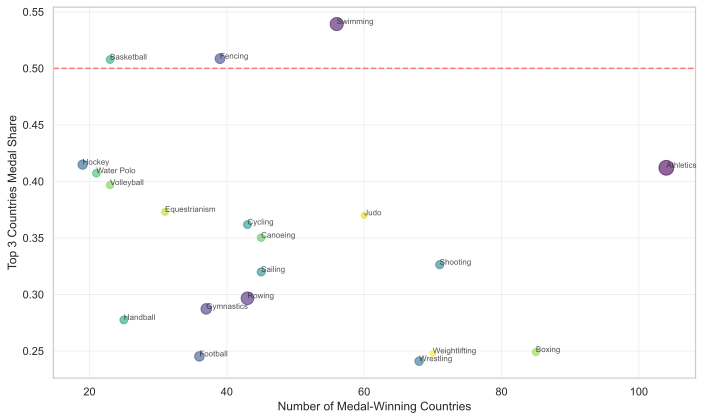
\includegraphics[width=0.5\textwidth]{fig4_sport_competition.pdf}
    \caption{Landscape of sports competition}
    \label{fig:sport_competition}
\end{figure}

Figure~\ref{fig:investment_matrix} categorizes sports events into four quadrants based on two dimensions: Top 3 countries monopoly and small Countries Medal Share. The upper-left quadrant represents “low monopoly-high opportunity” blue ocean events (green), characterized by fragmented competition and high breakthrough potential for smaller nations—ideal for emerging countries to prioritize. The lower-right quadrant denotes “high monopoly-low opportunity” red ocean events (red), dominated by leading powers; resource-constrained nations should approach these cautiously.

\begin{figure}[H]
    \centering
    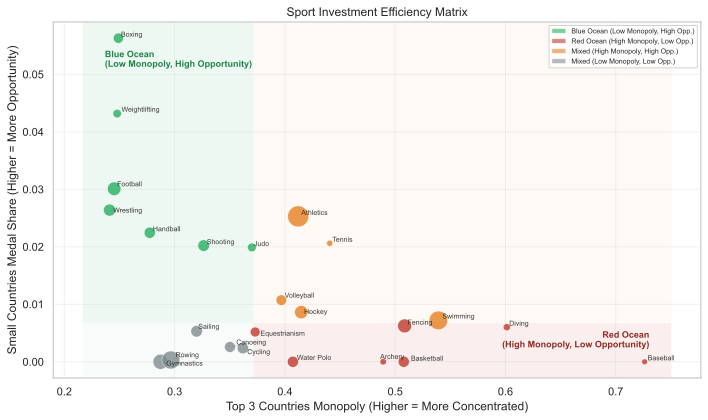
\includegraphics[width=0.5\textwidth]{fig5_investment_matrix.pdf}
    \caption{Investment efficiency matrix}
    \label{fig:investment_matrix}
\end{figure}

\subsection{Life Cycle of Sporting Powerhouses}

Sporting powerhouses follow a ~30-year lifecycle: 10-year rise (rapid growth), 10-year peak (high-level stability), and 10-year decline (share reduction). This pattern is confirmed by Russia's post-Soviet decline, Germany's reunification adjustment, and recent traditional powerhouses' relative decline. Early decline signals include continuous medal count reduction over 23 editions, significant gold medal ratio drops, and youth pipeline gaps. Strategic focus should shift from "broad layout" to "portfolio pruning," reallocating 15–20\% resources from stagnant projects to high-growth areas (e.g., urban/extreme sports). Figure~\ref{fig:market_share} illustrates this evolution via multiple line chart, showing the transition from US-Soviet hegemony to multipolarity in medal share.

\begin{figure}[H]
    \centering
    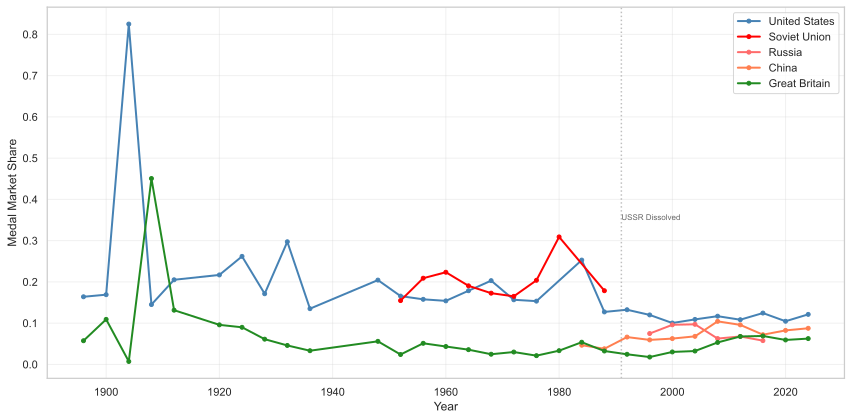
\includegraphics[width=0.5\textwidth]{fig6_market_share.pdf}
    \caption{Evolution of market share for powerhouses}
    \label{fig:market_share}
\end{figure}
Figure~\ref{fig:country_types} is based on K-means clustering results, classifying nations into two dimensions: "current strength" and "growth potential," and labeling differentiated strategic recommendations for different types of nations. Superpowers should focus on "maintenance and diversification," sporting powerhouses on "selecting excellence," rising nations on "targeted growth," emerging nations on "niche dominance," and developing nations on "solidifying the foundation."

\begin{figure}[H]
    \centering
    \includegraphics[width=0.5\textwidth]{fig7_country_types.pdf}
    \caption{Matrix of nation types and strategies}
    \label{fig:country_types}
\end{figure}
\section{Sensitivity Analysis}
To evaluate the robustness of the model to key settings, we conducted sensitivity analysis across three dimensions: regularization intensity, model category, and Bootstrap resampling. Our analysis reveals that the core predictions remain stable under variations in these parameters.
The stability of model performance is evident in Figure~\ref{fig:alpha_sensitivity}, where RMSE values remain consistently low (0.08--0.09) across a two-order-of-magnitude range of  $ \alpha $ . This demonstrates that the prediction results are insensitive to the choice of regularization parameter, with fluctuations only observed at extreme  $ \alpha $  values.

\begin{figure}[H]
    \centering
    \includegraphics[width=0.5\textwidth]{fig_sensitivity_alpha_rmse.pdf}
    \caption{RMSE stability across regularization intensity ( $ \alpha $ ) for Lasso and Ridge models.}
    \label{fig:alpha_sensitivity}
\end{figure}

Figure~\ref{fig:model_sensitivity} confirms that  $ R^2 $  values (0.93--0.95) remain highly consistent across all model categories (linear regression, regularized regression, and random forest), indicating that predictive performance is primarily determined by engineered features rather than modeling approach.

\begin{figure}[H]
    \centering
    \includegraphics[width=0.5\textwidth]{fig_sensitivity_model_r2.pdf}
    \caption{Model category comparison ( $ R^2 $  scores).}
    \label{fig:model_sensitivity}
\end{figure}

As shown in Figure~\ref{fig:bootstrap_sensitivity}, the RMSE distribution follows a tight normal curve (mean=0.085, std=0.003) with minimal dispersion, validating the model's stability under sample perturbation and the reliability of Bootstrap confidence intervals.
\begin{figure}[H]
    \centering
    \includegraphics[width=0.5\textwidth]{fig_sensitivity_bootstrap_rmse.pdf}
    \caption{RMSE distribution from 1000 Bootstrap resamples.}
    \label{fig:bootstrap_sensitivity}
\end{figure}

\section{Model Evaluation}
\subsection{Strengths}
The model framework of this study possesses the following advantages. First, it adopts a \textbf{data-driven approach} based on extensive historical data covering 128 years and 30 Olympic Games, ensuring the robustness of statistical inference. Second, the \textbf{feature engineering}  is comprehensive and systematic, constructing a multi-dimensional feature matrix that simultaneously captures both short-term momentum effects (lagged features) and medium-to-long-term stability (rolling averages), thereby enhancing the model's predictive power. Third, \textbf{uncertainty quantification} is sufficient; Bootstrap confidence intervals provide a probabilistic interpretation for point predictions, increasing the decision-making reference value of the results. Furthermore, to address the challenge of lacking direct coaching data, an \textbf{innovative indirect inference framework} combining change-point detection and DID was designed, demonstrating methodological creativity. Finally, the research findings have \textbf{strong practical applicability}, providing an actionable quantitative basis for the strategic planning and resource allocation of National Olympic Committees.

\subsection{Weaknesses}
This study also has the following limitations. First, regarding \textbf{data constraints}, the lack of direct coaching information necessitates reliance on indirect inference, which may overlook certain effects or attribute performance changes to incorrect causes. Second, regarding \textbf{sensitivity to assumptions}, the model assumes that historical patterns will continue into the future; in cases of major rule changes, geopolitical conflicts, or public health crises, the predictive effectiveness may be compromised. Third, regarding \textbf{predictive granularity}, the current predictions are at the national level; further refinement to the event level would provide more sophisticated decision support.


% --- References Section ---


\begin{thebibliography}{99}
\bibitem{1} Arrese, A. L., Urdiales, D. M., \& Izquierdo, D. M. (2013). Home advantage and sports performance: Evidence, causes, and psychological implications. \textit{Universitas Psychologica}, 12(3).
\bibitem{2} Baimbridge, M. (1998). Outcome uncertainty in sporting competition: The Olympic Games 1896–1996. \textit{Applied Economics Letters}, 5(3), 161–164.
\bibitem{3} Bredtmann, J., Crede, C. J.,\& Otten, S. (2016). Olympic medals: Does the past predict the future? \textit{Significance}, 13(3), 22–25.

\bibitem{4} Bernard, A. B., and Busse, M. R. (2004). Who wins the Olympic Games: Economic resources and medal totals. \textit{Review of Economics and Statistics}, 86(1), 413-417.
\bibitem{5}
Forrest, D., Sanz, I., \& Tena, J. D. (2010). Forecasting national team medal totals at the Summer Olympic Games. \textit{International Journal of Forecasting}, 26(3), 576–588.
\bibitem{6}
Lui, H. K., \& Suen, W. (2008). Men, money, and medals: An econometric analysis of the Olympic Games. \textit{Pacific Economic Review}, 13(1), 1–16.
\bibitem{7}
Balmer, N., Nevill, A., \& Williams, A. M. (2003). Modelling home advantage in the Summer Olympic Games. \textit{Journal of Sports Sciences}, 21(6), 469–478.

\bibitem{8}
Zhao, Y., \& Sun, Z. (2025). Medal prediction model based on machine learning. \textit{In Proceedings of the IEEE International Conference} (pp. 2408–2412). IEEE.
\end{thebibliography}

\begin{appendices}

\section{Feature List}

The complete list of features used in our prediction model:
\tiny
\begin{verbatim}
feature_columns = [
    'total_lag1',           # Previous edition's medals
    'total_lag2',           # Two editions ago's medals
    'gold_lag1',            # Previous edition's gold medals
    'total_rolling3_mean',  # Past 3 editions average
    'is_host',              # Host country indicator
    'total_events',         # Current edition's total events
    'participation_count',  # Number of participations
]
\end{verbatim}

\section{Statistical Test Details}

Detailed results of the t-test for host effect verification:
\begin{table}[H]
\centering
\begin{tabular}{lc}
\toprule
Statistic & Value \\
\midrule
Host Sample Size $n_1$ & 30 \\
Non-host Sample Size $n_2$ & 1,405 \\
Host Mean $\bar{X}_1$ & 66.9 \\
Non-host Mean $\bar{X}_2$ & 11.3 \\
Host Standard Deviation $s_1$ & 57.2 \\
Non-host Standard Deviation $s_2$ & 18.5 \\
t-statistic & 15.0 \\
p-value & < 0.001 \\
Cohen's $d$ & 2.77 (Large Effect) \\
\bottomrule
\end{tabular}
\end{table}

\end{appendices}
\end{document}

%% 
%% This work consists of these files mcmthesis.dtx,
%%                                   figures/ and
%%                                   code/,
%% and the derived files             mcmthesis.cls,
%%                                   mcmthesis-demo.tex,
%%                                   README,
%%                                   LICENSE,
%%                                   mcmthesis.pdf and
%%                                   mcmthesis-demo.pdf.
%%
%% End of file `mcmthesis-demo.tex'.
